\documentclass[10pt,a4paper]{article}% ===> this file was generated automatically by noweave --- better not edit it
\usepackage{pgf,tikz}
\usepackage{subfig}
\usepackage{amsmath}
\usepackage{amssymb}
\usepackage{noweb}
\usepackage{hyperref}
\usepackage{amsthm}
\usepackage{hyperref}
\setlength{\parskip}{3mm}
\newtheorem{axiom}{Axiom}
\newtheorem{definition}{Definition}
\newtheorem{comment}{Comment}
\newtheorem{example}{Example}
\newtheorem{lemma}{Lemma}
\newtheorem{prop}{Property}
\newtheorem{remark}{Remark}
\newtheorem{theorem}{Theorem}
\usetikzlibrary{arrows,fit,positioning}
\author{Dilawar Singh \\
Email : \texttt{dilawar@ee.iitb.ac.in}}
\title{Bipartite Graphs and Flow}
\begin{document}
\nwfilename{bipartite.snw}\nwbegindocs{1}\nwdocspar
\pagestyle{noweb}
\maketitle
\begin{abstract}
    
    We use several algorithms provided in {\Tt{}graph-tool]\ to\ find\ maximum\ flow\ in\nwnewline
\ \ \ \ bipartite\ graphs.\ Using\ [[unittest\nwendquote} module of python, we also write some
    tests which a correct program should pass. 

\end{abstract}

\nwenddocs{}\nwbegindocs{2}\section{First thing first}

Here is overall code-structure of this exercise.

\nwenddocs{}\nwbegincode{3}\moddef{*}\endmoddef\nwstartdeflinemarkup\nwenddeflinemarkup
\LA{}Import\RA{}
\LA{}Initialise\RA{}
\LA{}Subroutines\RA{}
\LA{}Test cases\RA{}
\LA{}Create flow networks\RA{}
\LA{}Calculate flow on networks\RA{}
\LA{}Save the work for posterity\RA{}
#ipshell() # if we want to drop into ipython
\eatline
\nwendcode{}\nwbegindocs{4}\nwdocspar
    Import {\Tt{}graphs-tool\nwendquote}. It is a wrapper written on boost-graph libraries
    written for python. It allows rapid prototyping. When an idea is tested, one
    can rewrite the whole thing in C++ when performance really matters.


\nwenddocs{}\nwbegincode{5}\moddef{Import}\endmoddef\nwstartdeflinemarkup\nwenddeflinemarkup
from graph_tool.all import * 
import array as ar
import numpy as np
import warnings as warn
\nwendcode{}\nwbegindocs{6}And we also need {\Tt{}Ipython\nwendquote} for better interaction with Hobbes \footnote{My
personal computer}.

\nwenddocs{}\nwbegincode{7}\moddef{Import}\plusendmoddef\nwstartdeflinemarkup\nwenddeflinemarkup
try:
    __IPYTHON__
except NameError:
    from IPython.Shell import IPShellEmbed
    ipshell = IPShellEmbed()
    # Now ipshell() will open IPython anywhere in the code
else:
    # Define a dummy ipshell() so the same code doesn't crash inside an
    # interactive IPython
    def ipshell(): pass

\nwendcode{}\nwbegindocs{8}And now we are ready to initialize a graph.

\nwenddocs{}\nwbegincode{9}\moddef{Initialise}\endmoddef\nwstartdeflinemarkup\nwenddeflinemarkup
g = Graph()

\nwendcode{}\nwbegindocs{10}\section{Bipartite graph}

A bipartite graph is a graph $G(V_{left}, V_{right}, E)$ where $V_{left}$ and
$V_{right}$ are two partition of vertices of graph $G$ such any edge $e \in E$
has one end point in $V_{left}$ and other is $V_{right}$. 


\begin{figure}[h]
\centering
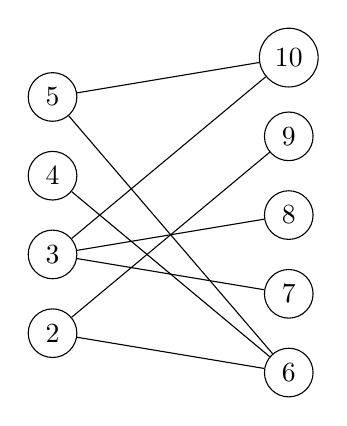
\begin{tikzpicture}
    \foreach \l in {2,3,4,5}
        \node[circle, draw] (\l) at (0, \l-2)  {$\l$};
    \foreach \r in {6,7,8,9,10}
        \node[circle, draw] (\r) at  (3, \r-6.5)  {$\r$};

    \path
        (2) edge (6) edge (9)
        (3) edge (10) edge (7) edge (8)
        (4) edge (6)
        (5) edge (10) edge (6);
\end{tikzpicture}
\caption{A biparite graph. There are many other 'varieties' of bipartite graph.}
\label{fig:generic_bipartite_graph}
\end{figure}

Many problems can be formulated using bipartite graphs. Given a bipartite graph,
We are interesting in 'matching'. A matching are edges from $V_{left}$ to
$V_{right}$ such that each vertex in one partition (the one which has less
vertices) is connected to one and only one vertex in another. We can form a
more intutive explanation of this problem.  Consider that of the left hand side
we have women (2,3,4,5) looking for men for marriage. Any edge form a vertex in
left (woman) to a vertex in right suggests a potential match. Figure out edges
which guarantees that each woman will get one man (ofcourse there will be
unmarried man, sigh).

In this excercise, we are not interested in such 'mundane' bipartite graphs.
Firstly, we'll have directed edges on vertices - both incoming and outgoing. We
are also not interested in matching (at least in this document). In addition to
direction of edges, we'll also put some number on an edge indication some
constraints on it. 

\begin{figure}[h]
\centering
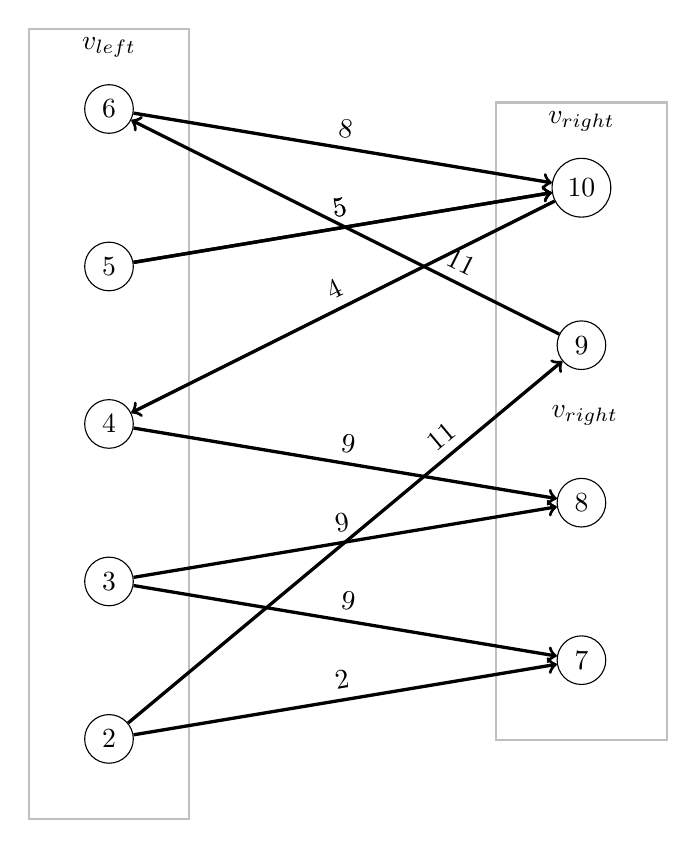
\begin{tikzpicture}
    \foreach \l in {2,3,4,5,6}
        \node[circle, draw] (\l) at (0, 2*\l-4)  {$\l$};
    \foreach \m in {7,8,9,10}
        \node[circle, draw] (\m) at  (6, 2*\m-13)  {$\m$};
%    \foreach \r in {11,12,13}
%        \node[circle, draw] (\r) at (12,2*\r-20) {$\r$};
    
    \node [draw=gray!50,inner sep=20pt
        ,thick,fit=(2) (3) (4) (5) (6)] (vl) {};
    \node[below] at (vl.north) {$v_{left}$};

     \node  [draw=gray!50,inner sep=20pt
        ,thick,fit=(7) (8) (9) (10)] (vr) {$v_{right}$};
    \node[below] at (vr.north) {$v_{right}$};
           
    \path[->, very thick]
        (2) edge node[sloped, above] {$2$} (7)
        (2) edge node[sloped, above, near end] {$11$} (9)
        (6) edge node[sloped, above] {$8$} (10)
        (9) edge node[sloped, above, near start] {$11$} (6)
        (5) edge node[sloped, above] {$5$} (10)
        (5) edge node[sloped, above] {$5$} (10)
        (10) edge node[sloped, above] {$4$} (4)
        (4) edge node[sloped, above] {$9$} (8)
        (3) edge node[sloped, above] {$9$} (8)
        (3) edge node[sloped, above] {$9$} (7)
    ;
\end{tikzpicture}
\caption{A biparite graph. Vertices are partioned into two, left and right.
There are only edges from one partition to other.}
\label{fig:bipartite_graph}
\end{figure}
 
An incoming edge will indicate 'in-flow' to a vertex while an outgoing edge will
indicate the 'out-flow' from  a vertex. A number on edge shows maximum capacity
of edge for such flow.

\nwenddocs{}\nwbegindocs{11}\section{Flow network of bipartite graph}

A flow network has a source vertex and a sink vertex. We add these two vertices
to our bipartite graph and put a very large (ideally infinite) capacity on all
edges which connects source and sink vertices to other vertices. We'll call such
a network a 'flow network' $F_G$ of bipartite graph $G$.

\begin{figure}[h]
\centering
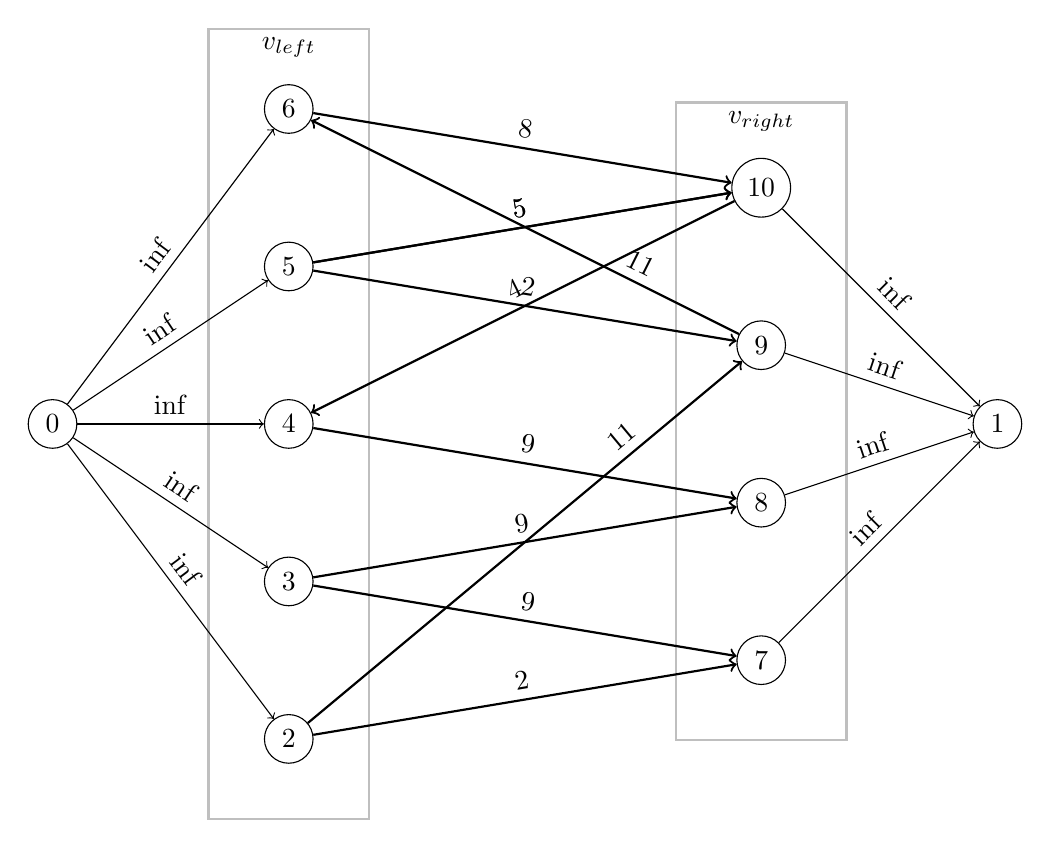
\begin{tikzpicture}
    \foreach \l in {2,3,4,5,6}
        \node[circle, draw] (\l) at (0, 2*\l-4)  {$\l$};
    \foreach \m in {7,8,9,10}
        \node[circle, draw] (\m) at  (6, 2*\m-13)  {$\m$};
%    \foreach \r in {11,12,13}
%        \node[circle, draw] (\r) at (12,2*\r-20) {$\r$};
    
    \node [draw=gray!50,inner sep=20pt
        ,thick,fit=(2) (3) (4) (5) (6)] (vl) {};
    \node[below] at (vl.north) {$v_{left}$};

     \node  [draw=gray!50,inner sep=20pt
        ,thick,fit=(7) (8) (9) (10)] (vr) {};
    \node[below] at (vr.north) {$v_{right}$};
    
    %% source and sink nodes.
    \node[draw, circle] (0) at (-3,4) {$0$};
    \node[draw, circle] (1) at (9,4) {$1$};


    \path[->, thick]
        (2) edge node[sloped, above] {$2$} (7)
        (2) edge node[sloped, above, near end] {$11$} (9)
        (6) edge node[sloped, above] {$8$} (10)
        (9) edge node[sloped, above, near start] {$11$} (6)
        (5) edge node[sloped, above] {$5$} (10)
        (5) edge node[sloped, above] {$2$} (9)
        (5) edge node[sloped, above] {$5$} (10)
        (10) edge node[sloped, above] {$4$} (4)
        (4) edge node[sloped, above] {$9$} (8)
        (3) edge node[sloped, above] {$9$} (8)
        (3) edge node[sloped, above] {$9$} (7)
    ;

    \path[->]
        (0)  edge node[sloped, above] {$\inf$} (2)
             edge node[sloped, above] {$\inf$} (3)
             edge node[sloped, above] {$\inf$} (4)
             edge node[sloped, above] {$\inf$} (5)
             edge node[sloped, above] {$\inf$} (6)
    ;
    \path[<-]
        
         (1) edge node[sloped, above] {$\inf$} (7)
             edge node[sloped, above] {$\inf$} (8)
             edge node[sloped, above] {$\inf$} (9)
             edge node[sloped, above] {$\inf$} (10)
    ;
\end{tikzpicture}
\caption{Flow network $F_G$ biparite graph $G$ of fig \ref{fig:bipartite_graph}.}
\label{fig:flow_bipartite_graph}
\end{figure}
 
If we find a maximum flow in such a network, we also find a minimum-cut. This
result is due to following theorem.

\begin{theorem}[Max flow min-cut theorem]

    In a given flow network $F$, the maximum value of flow from source to sink
    is equal to the minimum value of the capacities of all cuts which separates
    source from sink.

\end{theorem}


\nwenddocs{}\nwbegindocs{12}\section{Algorithms in {\Tt{}graph-tool\nwendquote}}

Given a biparite graph $G$, we construct a flow graph $F_G$. To automate this
task we write a function {\Tt{}bipToFlow\nwendquote}.

Each node in a flow graph $G$ has an index: 0 and 1 index is always reserved for
Source/sink nodes.  An optional {\Tt{}name\nwendquote} can also be attached to the graph
nodes. For bipartite graph, we need an additional property - 'if a vertex is in
left partition or in right partition'.

An edge in $G$ is more complicated. It has a maximum flow capacity {\Tt{}capcity\nwendquote} (integer),
flow value {\Tt{}flow\nwendquote} (integer) and a {\Tt{}name\nwendquote}.

\nwenddocs{}\nwbegincode{13}\moddef{Properties on edges and nodes}\endmoddef\nwstartdeflinemarkup\nwenddeflinemarkup
inf = 1000000 # infinite capacity.
vName = g.new_vertex_property("string") # name of the vertes (optional)
vLeft = g.new_vertex_property("bool") # if left or right node (left = True)
eName = g.new_edge_property("string") # name of an edge (optional)
eCaps = g.new_edge_property("int32_t") # capacity of edge
eFlow = g.new_edge_property("int32_t") # flow in edge 
\nwendcode{}\nwbegindocs{14}\nwdocspar

\nwenddocs{}\nwbegincode{15}\moddef{Properties on edges and nodes}\plusendmoddef\nwstartdeflinemarkup\nwenddeflinemarkup
# position of nodes
v_pos = g.new_vertex_property("vector<double>")

\nwendcode{}\nwbegincode{16}\moddef{Create flow networks}\endmoddef\nwstartdeflinemarkup\nwenddeflinemarkup
\LA{}Properties on edges and nodes\RA{}

\nwendcode{}\nwbegindocs{17}Our example (fig \ref{fig:flow_bipartite_graph}) has total 9 nodes (index 2 to
10).

\nwenddocs{}\nwbegincode{18}\moddef{Subroutines}\endmoddef\nwstartdeflinemarkup\nwenddeflinemarkup
#usage: 
#   addSourceSink(graph, left vertices, right vertices)
def addSourceSink(g, nLeft, nRight):
    g.add_vertex(nLeft+nRight+2) # additional source and sink
    for v in g.vertices():
        if (int(v) >= 2) & (int(v) <= (nLeft + 1)):
            vLeft[v] = True
            #print vLeft[v]
        else:
            vLeft[v] = False
            #print vLeft[v]
    return g
\eatline
\nwendcode{}\nwbegindocs{19}\nwdocspar
\nwenddocs{}\nwbegincode{20}\moddef{Create flow networks}\plusendmoddef\nwstartdeflinemarkup\nwenddeflinemarkup
# Our graph contains 9 vertices. 5 on left, 4 on right.
g = addSourceSink(g, 5, 4)

\nwendcode{}\nwbegindocs{21}Another soubroutine {\Tt{}addEdges\nwendquote} will be handy to attach edges to our graph.
We can pass edges as an list of pair $(in, out, caps)$ where $in$ is the
starting point of edge and $out$ is the end point of edge and $cap$ is the
capacity. For instance, in our example of \ref{fig:flow_bipartite_graph}, we can
capture all edges by writing $[(2,7,2), (2,9,11), (3,7,9), (3,8,9), (4,8,9),
(10,4,4), (5,10,5), (6,10,8), (9,6,5)]$.

\nwenddocs{}\nwbegincode{22}\moddef{Subroutines}\plusendmoddef\nwstartdeflinemarkup\nwenddeflinemarkup
def addEdges(g, edges):
    i = 0
    listEdges = list()
    for e in edges:
        listEdges.append(g.add_edge(g.vertex(int(e[0])), g.vertex(int(e[1]))))
        # and add capacity
        eCaps[listEdges[i]] = int(e[2])
        i += 1
    return g
\eatline
\nwendcode{}\nwbegindocs{23}\nwdocspar
\nwenddocs{}\nwbegincode{24}\moddef{Create flow networks}\plusendmoddef\nwstartdeflinemarkup\nwenddeflinemarkup
edges = [(2,7,2), (2,9,11), (3,7,9), (3,8,9), (4,8,9)
        , (10,4,4), (5,10,5), (5,9,2), (6,10,8), (9,6,5)]
g = addEdges(g, edges)

\nwendcode{}\nwbegindocs{25}Now last thing left, we have to attach edges of infinite capacity to turn it
into a flow network. We could have done it in {\Tt{}addEdges\nwendquote} also but I like
making one function for one job even if the a significant part is repetitive.
However there is a huge disadvantage doing it for a big graph.

\nwenddocs{}\nwbegincode{26}\moddef{Subroutines}\plusendmoddef\nwstartdeflinemarkup\nwenddeflinemarkup
def attachInfCapEdges(g):
    for v in g.vertices():
        if int(v) >= 2:
            if vLeft[v] == True :
                e = g.add_edge(g.vertex(0), v)
                eCaps[e] = inf
            else:
                e = g.add_edge(v, g.vertex(1))
                eCaps[e] = inf
    return g
\eatline
\nwendcode{}\nwbegindocs{27}\nwdocspar
\nwenddocs{}\nwbegincode{28}\moddef{Create flow networks}\plusendmoddef\nwstartdeflinemarkup\nwenddeflinemarkup
g = attachInfCapEdges(g)


\nwendcode{}\nwbegindocs{29}Now we should save this work. We may like to use this graph again some day.
Before saving this graph, we should also turn edge and vertex properties to the
property of graph.


\nwenddocs{}\nwbegincode{30}\moddef{Save the work for posterity}\endmoddef\nwstartdeflinemarkup\nwenddeflinemarkup
# covert properties to global properties.
g.edge_properties["caps"] = eCaps # capacity
g.vertex_properties["lr"] = vLeft # left or right
g.save("graphs/bipartite.xml.gz")
# and print also.
graph_draw(g #, pos=v_pos
    , vprops=\{"label":g.vertex_index\}
    , eprops = \{"label":eCaps\}
    , sep = 1.0, output="figs/bip__flow.pdf")

\nwendcode{}\nwbegindocs{31}Now, it's time to solve this network. This package {\Tt{}graph-tool\nwendquote} gives 3 well
known algorithms: {\Tt{}edmond{\_}karp{\_}max{\_}flow\nwendquote}, {\Tt{}push{\_}relable{\_}max{\_}flow\nwendquote}, and
{\Tt{}boykov{\_}kolmogorov{\_}max{\_}flow\nwendquote}. Lets write some functions to automate this task.

\nwenddocs{}\nwbegincode{32}\moddef{Subroutines}\plusendmoddef\nwstartdeflinemarkup\nwenddeflinemarkup
def edmondKarp(graph, prop):
    src, tgt = graph.vertex(0), graph.vertex(1)
    res = edmonds_karp_max_flow(graph, src, tgt, prop)
    res.a = prop.a - res.a
    max_flow = sum(res[e] for e in tgt.in_edges())
    return max_flow, res.a
\eatline
\nwendcode{}\nwbegindocs{33}\nwdocspar
\nwenddocs{}\nwbegincode{34}\moddef{Subroutines}\plusendmoddef\nwstartdeflinemarkup\nwenddeflinemarkup
def pushRelabel(graph, prop):
    src, tgt = graph.vertex(0), graph.vertex(1)
    res = push_relabel_max_flow(graph, src, tgt, prop)
    res.a = prop.a - res.a
    max_flow = sum(res[e] for e in tgt.in_edges())
    return max_flow, res.a
\eatline
\nwendcode{}\nwbegindocs{35}\nwdocspar
\nwenddocs{}\nwbegincode{36}\moddef{Subroutines}\plusendmoddef\nwstartdeflinemarkup\nwenddeflinemarkup
def kolmogorov(graph, prop):
    src, tgt = graph.vertex(0), graph.vertex(1)
    res = boykov_kolmogorov_max_flow(graph, src, tgt, prop)
    # here we have a bug. res returned by above method does not have the same length
    # as others.
    if res.a.size == prop.a.size:
         res.a = prop.a - res.a
    else:
        warn.warn("Loop found here. This method can't handle it")
        return -1, res.a
    max_flow = sum(res[e] for e in src.out_edges())
    return max_flow, res.a
\nwendcode{}\nwbegindocs{37}\nwdocspar

\nwenddocs{}\nwbegincode{38}\moddef{Calculate flow on networks}\endmoddef\nwstartdeflinemarkup\nwenddeflinemarkup

\nwendcode{}\nwbegindocs{39}Now it is a good time for some testing frameworks. Pyhton procides a
good testing module {\Tt{}unittest\nwendquote}.
\nwenddocs{}\nwbegincode{40}\moddef{Import}\plusendmoddef\nwstartdeflinemarkup\nwenddeflinemarkup
import unittest

\nwendcode{}\nwbegindocs{41}We now create a class with some properties, to which we'll add new
properties as we go along on our journey.

\nwenddocs{}\nwbegincode{42}\moddef{Test cases}\endmoddef\nwstartdeflinemarkup\nwenddeflinemarkup
class GraphTestClass(unittest.TestCase):  
    # this is responsible in setting up the test-bench.
    def setUp(self): pass

    def createData(self, g, prop):
        self.flow1, self.res1 = edmondKarp(g, prop)
        self.flow2, self.res2 = pushRelabel(g, prop)
        self.flow3, self.res3 = kolmogorov(g, prop)
 
class TestForEquality(GraphTestClass):
    \LA{}Add tests\RA{}

\eatline
\nwendcode{}\nwbegindocs{43}\nwdocspar
\nwenddocs{}\nwbegindocs{44}Before we proceed, it's not a bad idea to define some trivial properties. For
example, check if all three available algorithms are producing same answers.

\nwenddocs{}\nwbegincode{45}\moddef{Add tests}\endmoddef\nwstartdeflinemarkup\nwenddeflinemarkup
# for graph g
def testEqualG(self):
    self.createData(g, eCaps)
    if self.flow1 > 0 and self.flow2 > 0 and self.flow3 > 0 : 
        self.assertEqual(self.flow1, self.flow2)
        self.assertEqual(self.flow2, self.flow3)
        self.assertEqual(self.res1.all(), self.res2.all())
        self.assertEqual(self.res2.all(), self.res3.all())
    else:
        warn.warn("Negative Flow. One of more method is unsuitable.")
\nwendcode{}\nwbegindocs{46}\section{Solution}
\nwenddocs{}\nwbegincode{47}\moddef{Calculate flow on networks}\plusendmoddef\nwstartdeflinemarkup\nwenddeflinemarkup
flow1, res1 = edmondKarp(g, eCaps)
print flow1, res1
flow2, res2 = pushRelabel(g, eCaps)
print flow2, res2
flow3, res3 = kolmogorov(g, eCaps)
print flow3, res3
\nwendcode{}\nwbegindocs{48}\nwdocspar
\end{document}
\nwenddocs{}
